\subsection{Winkelmodulation (FM/PM) S. 66}
\textbf{Idee:} Die Amplitude bleibt konstant $A_c$, die Nachricht $m(t)$ steckt \textbf{nur im Winkel} des Cosinus. Vorteil gegenüber AM: grössere Störfestigkeit. Nachteil: grössere Bandbreite.

\subsubsection{Grundform -- alles wird an $\varphi(t)$ abgelesen}
\boxedeq{
	x(t) &= A_c \cdot \cos\big(\theta(t)\big) \qquad \text{mit} \qquad \theta(t) = \underbrace{\omega_c t}_{\text{Träger}} + \underbrace{\varphi(t)}_{\text{Phasenabweichung}}
}

\begin{tabularx}{\linewidth}{>{\raggedright\arraybackslash}p{.30\linewidth} >{\raggedright\arraybackslash}X}
	\textbf{Momentanphase} $\theta(t)$ [rad] & ganzes Argument des Cosinus \\
	\textbf{Phasenabweichung} $\varphi(t)$ [rad] & $\theta(t) - \omega_c t$: der Teil, der die Nachricht trägt \\
	\textbf{Momentankreisfrequenz} $\omega_i(t)$ & $\displaystyle \omega_i(t) = \frac{\diff\theta(t)}{\diff t} = \omega_c + \frac{\diff\varphi(t)}{\diff t}$ \qquad $\displaystyle f_i(t) = \frac{\omega_i(t)}{2\pi}$ \\[8pt]
	\textbf{Frequenzabweichung} & $\displaystyle \frac{\diff\varphi(t)}{\diff t}$ \quad (= $\omega_i - \omega_c$, also \textbf{ohne} Träger) \\[8pt]
	\textbf{Max. Phasenabweichung} (Phasenhub) & $\displaystyle \Delta\varphi = \max\big|\varphi(t)\big|$ \quad [rad] \\[6pt]
	\textbf{Max. Frequenzabweichung} (Frequenzhub) & $\displaystyle \Delta\omega = \max\left|\frac{\diff\varphi(t)}{\diff t}\right|$ \quad [rad/s] \qquad $\displaystyle \Delta f = \frac{\Delta\omega}{2\pi}$ \quad [Hz] \\
\end{tabularx}

\vspace{.2cm}
\textbf{Merke:} Die Momentanfrequenz ist die \textbf{Ableitung der Phase}. Konstante Phase $\Rightarrow$ $f_i = f_c$. Phase $\sim t^2$ $\Rightarrow$ $f_i$ steigt linear (Chirp).

\subsubsection{PM und FM im Vergleich}
Unterschied: \textbf{wo} $m(t)$ hineingesteckt wird. PM: $m(t)$ ist proportional zur \emph{Phase}. FM: $m(t)$ ist proportional zur \emph{Frequenz}, die Phase ist deshalb das \emph{Integral} von $m(t)$.

{\renewcommand{\arraystretch}{2.1}
\begin{tabularx}{\linewidth}{|>{\raggedright\arraybackslash}p{.24\linewidth}|>{\centering\arraybackslash}X|>{\centering\arraybackslash}X|}
	\hline
	& \textbf{Phasenmodulation PM} & \textbf{Frequenzmodulation FM} \\ \hline
	Signal & $x_{PM}(t) = A_c\cos\big(\omega_c t + k_P\, m(t)\big)$ & $\displaystyle x_{FM}(t) = A_c\cos\Big(\omega_c t + k_F \int_{-\infty}^{t} m(\tau)\diff\tau\Big)$ \\ \hline
	Phasenabweichung $\varphi(t)$ & $\varphi(t) = k_P \cdot m(t)$ & $\displaystyle \varphi(t) = k_F \int_{-\infty}^{t} m(\tau)\diff\tau$ \\ \hline
	Frequenzabweichung $\frac{\diff\varphi}{\diff t}$ & $\displaystyle \frac{\diff\varphi}{\diff t} = k_P \cdot \frac{\diff m(t)}{\diff t}$ & $\displaystyle \frac{\diff\varphi}{\diff t} = k_F \cdot m(t)$ \\ \hline
	Momentankreisfrequenz & $\displaystyle \omega_i(t) = \omega_c + k_P \cdot \frac{\diff m(t)}{\diff t}$ & $\omega_i(t) = \omega_c + k_F \cdot m(t)$ \\ \hline
	Phasenhub $\Delta\varphi$ & $k_P \cdot \max|m(t)|$ & $\displaystyle k_F \cdot \max\Big|\int m(\tau)\diff\tau\Big|$ \\ \hline
	Frequenzhub $\Delta\omega$ & $\displaystyle k_P \cdot \max\left|\frac{\diff m(t)}{\diff t}\right|$ & $k_F \cdot \max|m(t)|$ \\ \hline
	Konstante & $k_P$ = Phasenhubkonstante [rad] (pro Einheit von $m$) & $k_F$ = Frequenzhubkonstante [rad/s] (pro Einheit von $m$) \\ \hline
	\textbf{Rückwärts:} $m(t)$ aus $\varphi(t)$ & \efbox[linecolor=red]{$\displaystyle m(t) = \frac{\varphi(t)}{k_P}$} & \efbox[linecolor=red]{$\displaystyle m(t) = \frac{1}{k_F}\cdot\frac{\diff\varphi(t)}{\diff t}$} \\ \hline
\end{tabularx}}

\vspace{.2cm}
\begin{minipage}[t]{.48\linewidth}
	\centering PM im Zeitbereich\\
	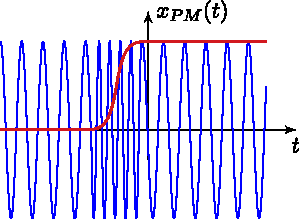
\includegraphics[width=.9\linewidth]{chapters/06_amplitudenmodulation/figures/xpm.pdf}
\end{minipage}\hfill
\begin{minipage}[t]{.48\linewidth}
	\centering FM im Zeitbereich\\
	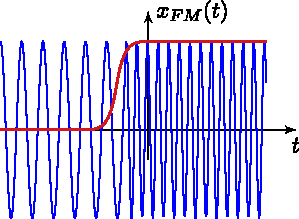
\includegraphics[width=.9\linewidth]{chapters/06_amplitudenmodulation/figures/xfm.pdf}
\end{minipage}

\paragraph{Zeitverschiebung und Phase}
Eine Phasenabweichung $\varphi$ entspricht einer Zeitverschiebung $\Delta T$ des Trägers: $\varphi = 2\pi \cdot \frac{\Delta T}{T_c} = 2\pi f_c \cdot \Delta T$. Damit z.B. $k_P = 2\pi \cdot \frac{t_{delay,max}}{T_c}$ (bei normiertem $\max|m| = 1$).

\subsubsection{Äquivalenz PM und FM}
Am Signal allein sieht man \textbf{nicht}, ob PM oder FM vorliegt: beide haben die Form $A_c\cos(\omega_c t + \varphi(t))$. Erst die Annahme (PM mit $k_P$ oder FM mit $k_F$) legt $m(t)$ fest.

% \begin{center}
% \begin{tikzpicture}[font=\small, >=stealth]
% 	\node[draw, rounded corners, fill=lightgray, align=center] (x) at (0,0) {$x(t)$\\ auf Form $A_c\cos(\theta(t))$};
% 	\node[draw, rounded corners, fill=lightgray, align=center] (p) at (4.6,0) {$\varphi(t) = \theta(t) - \omega_c t$};
% 	\node[draw, rounded corners, fill=primary!10, align=center] (pm) at (9.6,0.8) {\textbf{PM:} $m(t) = \varphi(t)\,/\,k_P$};
% 	\node[draw, rounded corners, fill=accent2!15, align=center] (fm) at (9.6,-0.8) {\textbf{FM:} $m(t) = \varphi'(t)\,/\,k_F$};
% 	\draw[->, thick] (x) -- (p);
% 	\draw[->, thick] (p.east) -- (pm.west);
% 	\draw[->, thick] (p.east) -- (fm.west);
% \end{tikzpicture}
% \end{center}

\begin{minipage}{.55\linewidth}
	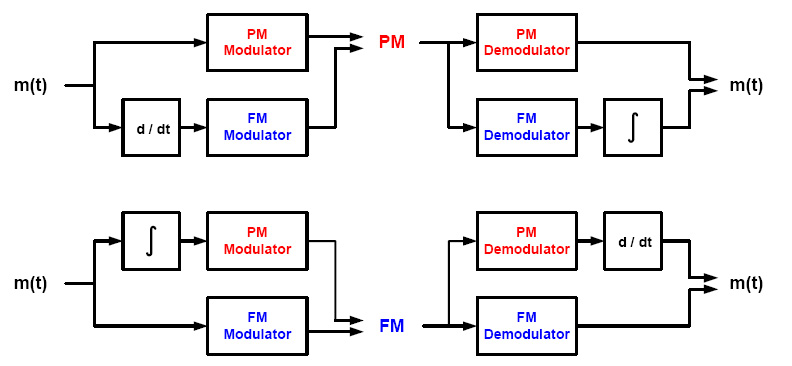
\includegraphics[width=\linewidth]{chapters/06_amplitudenmodulation/figures/PMundFM.png}
\end{minipage}\hfill
\begin{minipage}{.42\linewidth}
	\textbf{FM mit PM-Modulator:} $m(t)$ zuerst integrieren, dann PM.\\
	\textbf{PM mit FM-Modulator:} $m(t)$ zuerst differenzieren, dann FM.
\end{minipage}

\subsubsection{Einton-Winkelmodulation (sinusförmiges $m(t)$)}
Ansatz des Skripts, so dass in beiden Fällen $\varphi(t) = \beta\sin(\omega_m t)$ herauskommt:

{\renewcommand{\arraystretch}{2.1}
\begin{tabularx}{\linewidth}{|>{\raggedright\arraybackslash}p{.24\linewidth}|>{\centering\arraybackslash}X|>{\centering\arraybackslash}X|}
	\hline
	& \textbf{PM:} $m(t) = A_m\sin(\omega_m t)$ & \textbf{FM:} $m(t) = A_m\cos(\omega_m t)$ \\ \hline
	$\varphi(t)$ & $k_P A_m \sin(\omega_m t)$ & $\displaystyle \frac{k_F A_m}{\omega_m}\sin(\omega_m t)$ \\ \hline
	Modulationsindex $\beta$ & $\beta_{PM} = k_P A_m$ \quad (unabhängig von $f_m$) & $\displaystyle \beta_{FM} = \frac{k_F A_m}{\omega_m}$ \quad ($\sim 1/f_m$) \\ \hline
	Frequenzhub $\Delta f$ & $\displaystyle \frac{k_P A_m \omega_m}{2\pi} = \beta f_m$ \quad ($\sim f_m$) & $\displaystyle \frac{k_F A_m}{2\pi}$ \quad (unabhängig von $f_m$) \\ \hline
\end{tabularx}}

\vspace{.2cm}
\boxedeq{
	\varphi(t) = \beta\sin(\omega_m t) \quad\Longrightarrow\quad \Delta\varphi = \beta \qquad \Delta\omega = \beta\,\omega_m \qquad \beta = \frac{\Delta\omega}{\omega_m} = \frac{\Delta f}{f_m}
}
$\beta$ ist nur für Eintonsignale definiert und ist \textbf{gleich dem Phasenhub} $\Delta\varphi$.

\subsubsection{Kochrezept für Aufgaben}
\begin{enumerate}
	\setlength{\itemsep}{1pt}
	\item \textbf{Auf Form bringen:} $x(t) = A_c\cos(\theta(t))$. Falls $x(t)$ als Summe gegeben ist, Additionstheoreme:\\
	$\cos\alpha\cos\beta + \sin\alpha\sin\beta = \cos(\alpha-\beta)$ \qquad $\cos\alpha\cos\beta - \sin\alpha\sin\beta = \cos(\alpha+\beta)$
	\item \textbf{Träger abtrennen:} den Term $\sim t$ als $\omega_c t$ nehmen, Rest ist $\varphi(t)$. Achtung: $f_c = \omega_c / 2\pi$, z.B. $\cos(10^8\pi t)$ $\Rightarrow$ $f_c = \qty{50}{\MHz}$.
	\item \textbf{Momentanfrequenz:} $\omega_i(t) = \frac{\diff\theta}{\diff t}$, \; $f_i(t) = \frac{\omega_i}{2\pi}$. Konstant, linear oder sinusförmig um $f_c$?
	\item \textbf{Hübe:} $\Delta\varphi = \max|\varphi|$, \; $\Delta\omega = \max|\varphi'|$, \; $\Delta f = \Delta\omega/2\pi$. Bei $\varphi = \beta\sin(\omega_m t)$: $\Delta\varphi = \beta$, \; $\Delta f = \beta f_m$.
	\item \textbf{Nachricht:} PM $\Rightarrow m = \varphi/k_P$, \; FM $\Rightarrow m = \varphi'/k_F$ (Tabelle oben).
	\item \textbf{Bandbreite:} Carson $B = 2(\Delta f + f_m) = 2(\beta + 1) f_m$ (siehe unten).
\end{enumerate}

\paragraph{Beispiel} $x(t) = 5\cos\big(2\pi\cdot 10^6 t + 3\sin(2\pi\cdot 200\, t)\big)$
\begin{itemize}
	\setlength{\itemsep}{0pt}
	\item $f_c = \qty{1}{\MHz}$, \; $\varphi(t) = 3\sin(2\pi\cdot 200\,t)$ $\Rightarrow$ $\Delta\varphi = \beta = 3$ rad, \; $f_m = \qty{200}{\Hz}$
	\item $f_i(t) = \frac{1}{2\pi}\frac{\diff\theta}{\diff t} = 10^6 + 3\cdot 200\cos(2\pi\cdot 200\,t)$ Hz $\Rightarrow$ $\Delta f = \qty{600}{\Hz}$ (schwankt zwischen $f_c \pm \qty{600}{\Hz}$)
	\item als PM mit $k_P = 2$: $m(t) = \varphi/k_P = 1.5\sin(2\pi\cdot 200\,t)$
	\item als FM mit $k_F = 2\pi\cdot 300$: $m(t) = \varphi'/k_F = \frac{3\cdot 2\pi\cdot 200}{2\pi\cdot 300}\cos(2\pi\cdot 200\,t) = 2\cos(2\pi\cdot 200\,t)$
	\item Carson: $B = 2(600 + 200) = \qty{1.6}{\kHz}$
\end{itemize}

\subsubsection{Winkelmodulation ist nicht linear}
\begin{tabularx}{\linewidth}{>{\raggedright\arraybackslash}p{.18\linewidth} >{\raggedright\arraybackslash}X}
	\textbf{DSB-SC (linear):} & $A_c\,(m_1 + m_2)\cos(\omega_c t) = x_{DSB1}(t) + x_{DSB2}(t)$ \quad $\checkmark$ \\
	\textbf{PM (nicht linear):} & $A_c\cos\big(\omega_c t + k_P(m_1 + m_2)\big) \neq A_c\cos(\omega_c t + k_P m_1) + A_c\cos(\omega_c t + k_P m_2)$ \\
\end{tabularx}\\
Die Summe der Nachrichten steckt im \emph{Argument} des Cosinus, nicht davor. Deshalb gilt der Überlagerungssatz nicht, und das Spektrum ist nicht einfach das verschobene $M(\omega)$.

\subsubsection{Äquivalente Basisbanddarstellung}
\begin{minipage}{.45\linewidth}
	Äquivalente Basisbanddarstellung $x_{eq}(t) = e^{j\varphi(t)}$: Punkte auf dem Einheitskreis (Amplitude konstant)
	\newline

	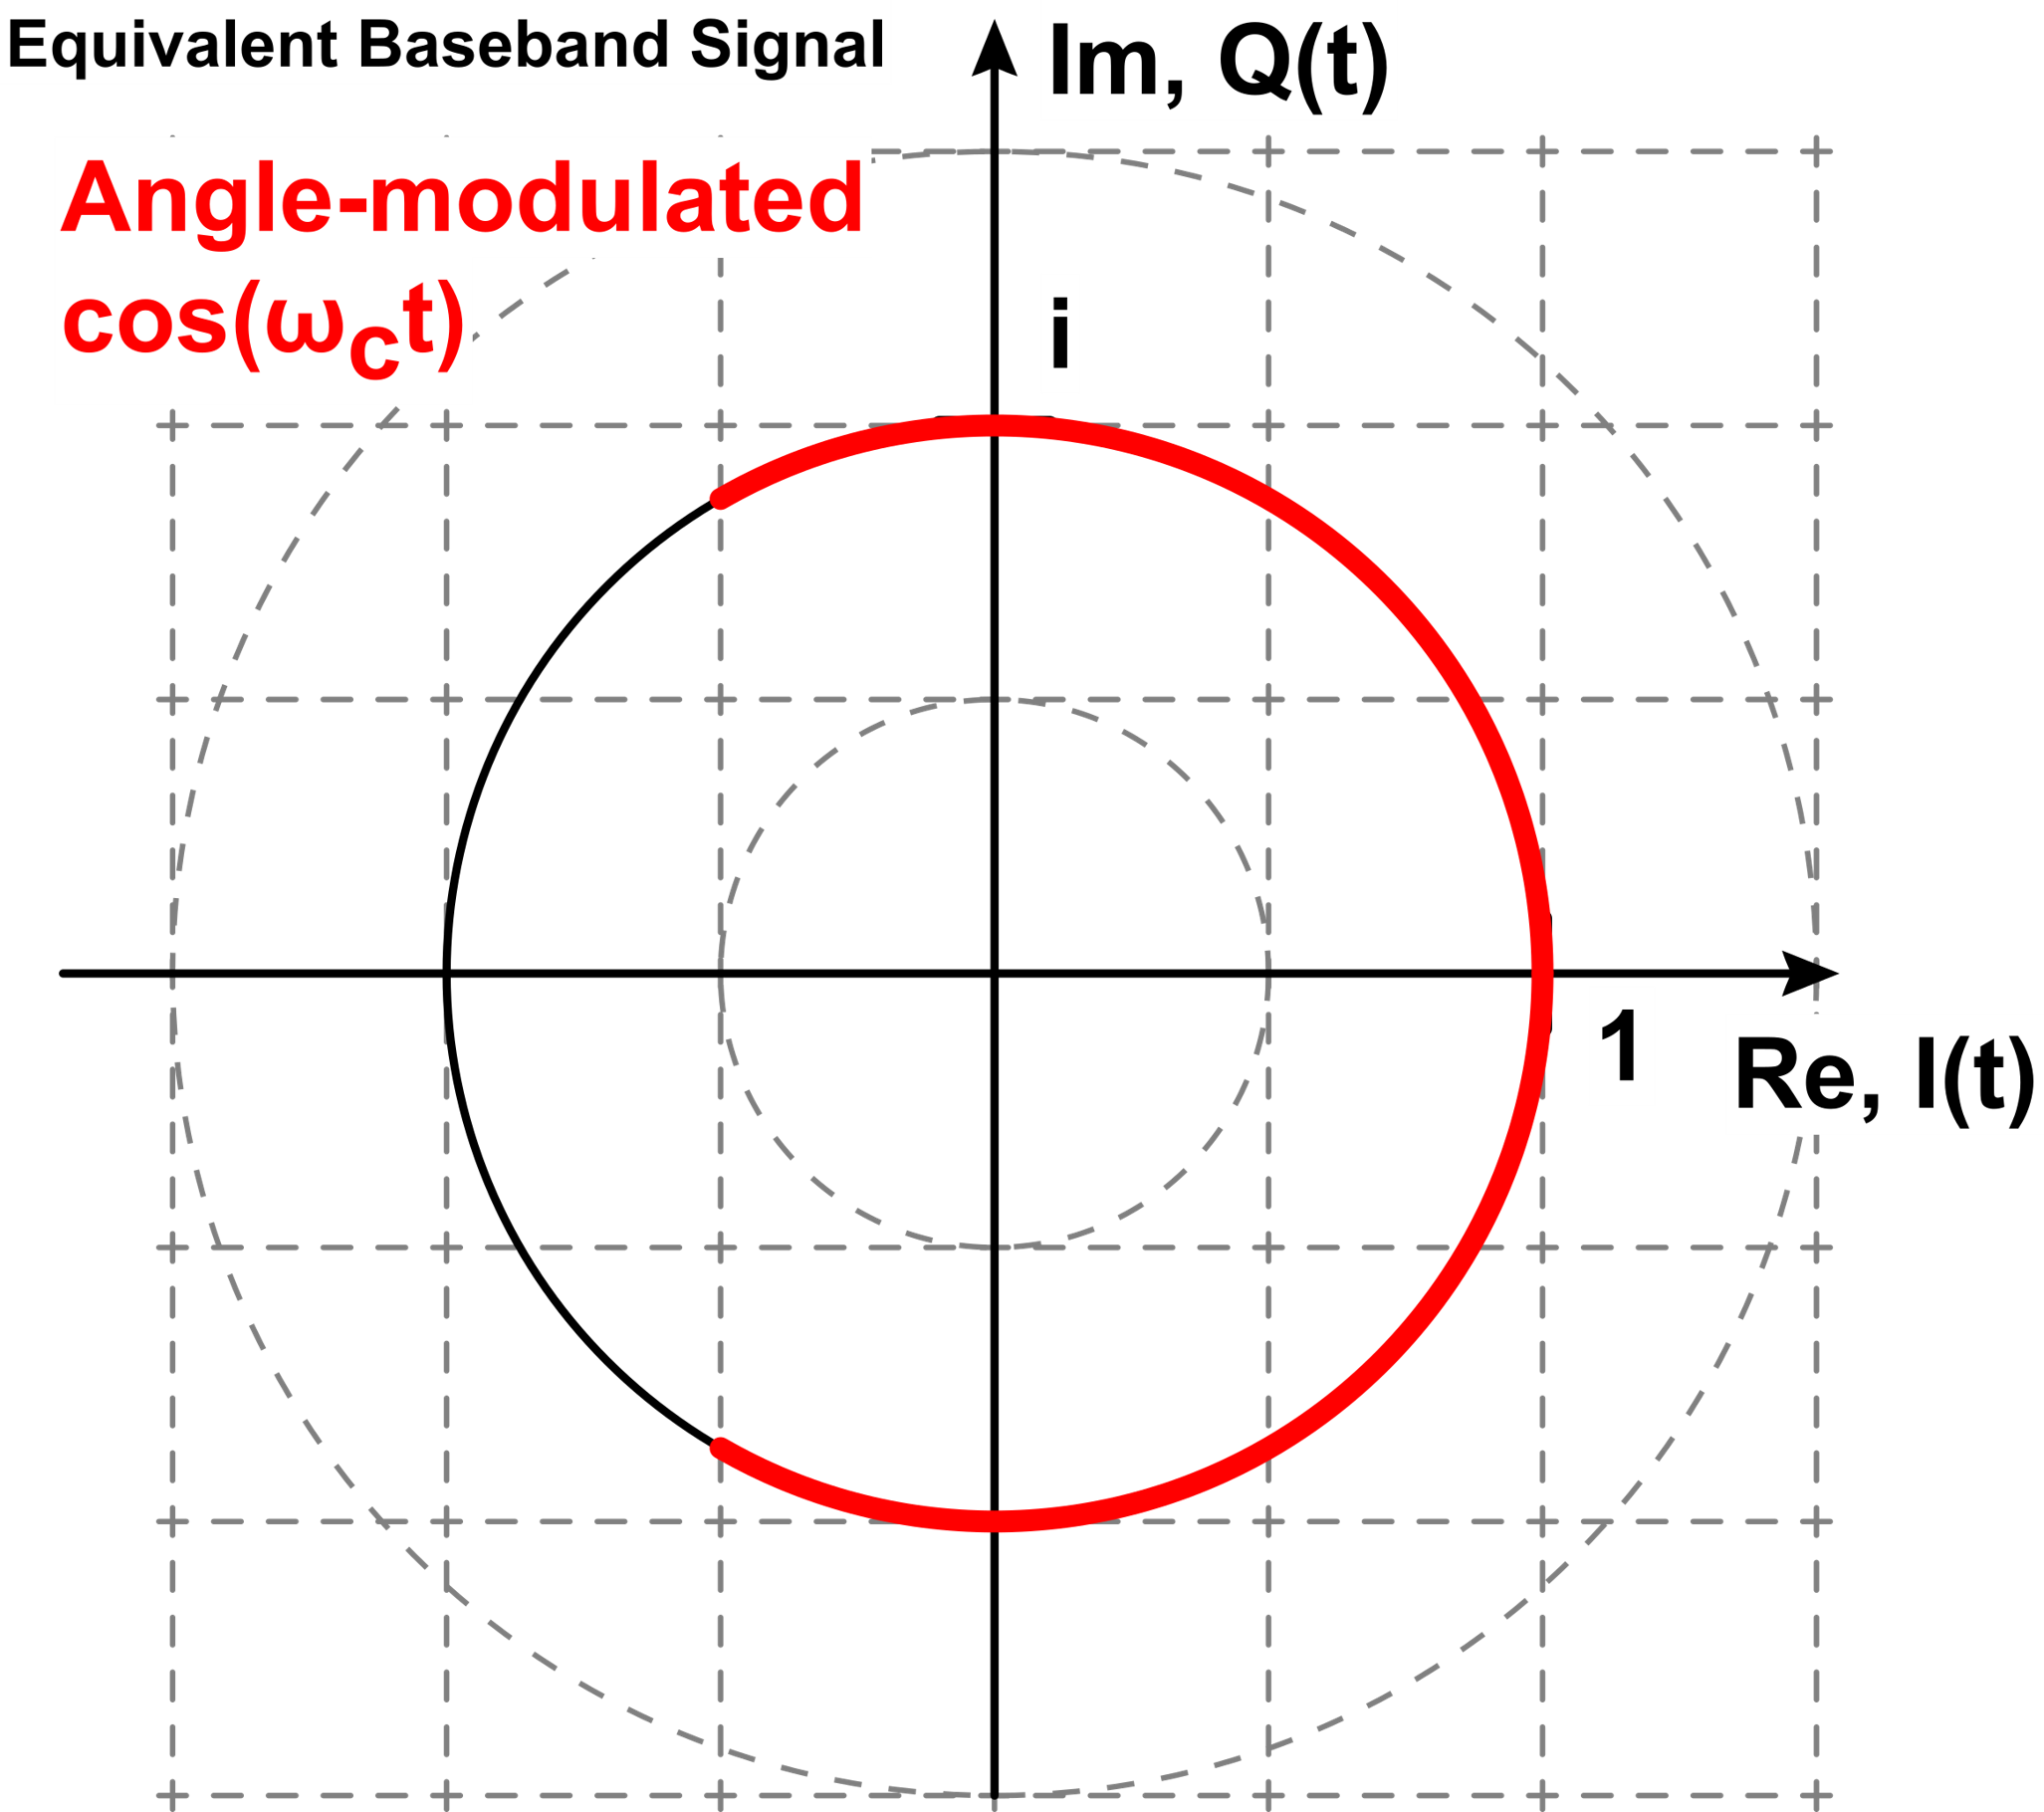
\includegraphics[width=.6\linewidth]{chapters/06_amplitudenmodulation/figures/PM_zeiger.png}
\end{minipage} \hspace{.1\linewidth}
\begin{minipage}{.45\linewidth}

	Zeigerdiagramm des winkelmodulierten Trägersignals

	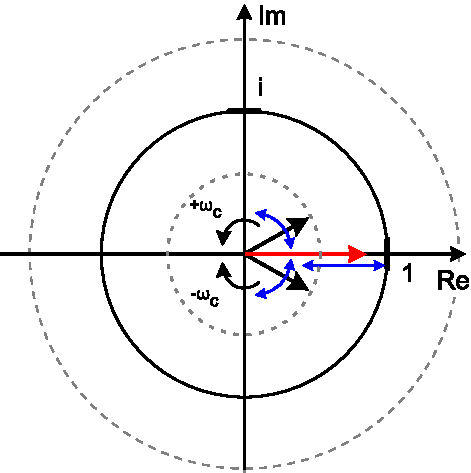
\includegraphics[width=.6\linewidth]{chapters/06_amplitudenmodulation/figures/abbildung5_26.pdf}
\end{minipage}

\subsubsection{Spektrum der Winkelmodulation S. 70}
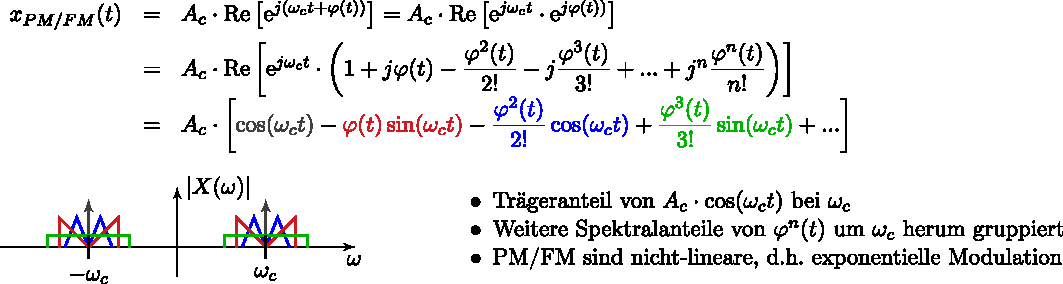
\includegraphics[width=\linewidth]{chapters/06_amplitudenmodulation/figures/spektrumWinkelmodulation.pdf}

\subsubsection{Kleinhub Winkelmodulation S. 70}
\begin{table}[H]
	\begin{tabularx}{\linewidth}{m{.65\linewidth} m{.35\linewidth}}
		\begin{minipage}{\linewidth}
				Kleinhubmodulation funktioniert in der Praxis bei ca: \efbox[linecolor=red]{$|\varphi(t)| < 0.2 \text{ rad}$} bzw. 10 bis 12 Grad. \\
				Dann gilt: \efbox[linecolor=red]{$x_{NB\varphi M}(t) \approx A_c \cdot \cos(\omega_c t) - A_c \cdot \varphi(t)\cdot \sin(\omega_ct)$} \\
				\textbf{Demodulation:} mit kohärentem Produktdetektor\\ $\rightarrow x_{NB-PM/FM}(t)\cdot (-\sin(\omega_c t))$ \\
				Bild rechts: äquivalente Basisbanddarstellung des Signals\\ $x_{NB-PM}(t) = 0.05 \cdot \sin(2\pi \cdot 200 t) + 1\cdot \sin(2\pi \cdot 1000 t)$\\
				Wichtig ist nur, dass die Signalamplitude im Vergleich zur Trägeramplitude sehr klein ist (siehe Formeln zu Beginn des Kapitels)
		\end{minipage}
		&
		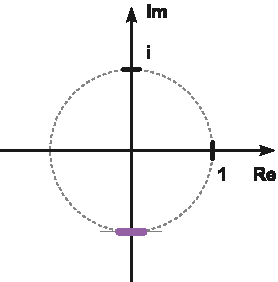
\includegraphics[width=.8\linewidth]{chapters/06_amplitudenmodulation/figures/eqBase_NBAM.pdf}
	\end{tabularx}
\end{table}

\paragraph{Spektrum S. 70}
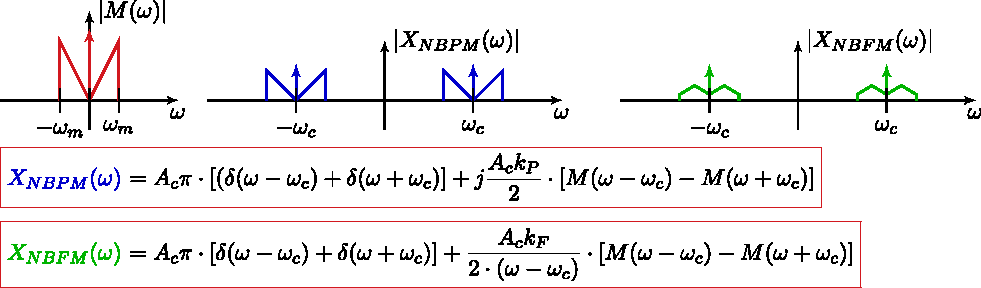
\includegraphics[width=.8\linewidth]{chapters/06_amplitudenmodulation/figures/spektrumNB_PM.pdf}\\
\textbf{Vergleich AM und NB-PM:} Qualitativ gilt für die Amplitudenspektren $|X_{AM}(\omega)| = |X_{NBPM}(\omega)|$ (Träger und 2 Seitenbänder). Bei AM sind die Seitenbänder in Phase zum Träger, bei NB-PM orthogonal dazu.

\subsubsection{Grosshub Winkelmodulation S. 71}
WideBand Angle Modulation, siehe auch Skript Seite 67 \hspace{.3cm} \efbox[linecolor=red]{$|\varphi (t)| > 1 \text{ rad}$}
	\begin{list}{$\bullet$}{\setlength{\itemsep}{0cm} \setlength{\parsep}{0cm} 	\setlength{\topsep}{0cm}}
	\item nicht lineare Terme von $\varphi (t)$ nicht mehr vernachlässigbar
	\item analytische Bestimmung des Spektrums nur noch für Eintonsignale durchführbar
	\item Überlagerungssatz nicht mehr gültig
	\item $x_{FM/PM}$ ist zu $m(t)$ stark nicht linear
	\item im Spektrum treten Faltungen $M * M * \dots$ auf: das Spektrum wird breiter als $2B_m$
\end{list}
\begin{table}[H]
	\begin{tabularx}{\linewidth}{m{.7\linewidth} m{.3\linewidth}}
		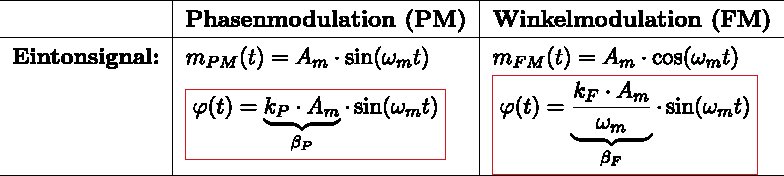
\includegraphics{chapters/06_amplitudenmodulation/figures/WB_PM.pdf}
		&
		\begin{minipage}{.9\linewidth}
			\begin{center}
				Modulationsindex:\\
				\efbox[linecolor=red]{$\beta = \frac{\Delta \omega}{\omega_m} = \Delta\varphi$}\\
				Ist nur für Eintonsignale definiert!\\
				\efbox[linecolor=red]{$\Delta T=\frac{1}{f_c}\cdot \frac{\beta}{2\pi}$} \\
				max. Zeitverschiebung des Trägers
			\end{center}
		\end{minipage}
	\end{tabularx}
\end{table}

\subsubsection{Spektrum Einton-Winkelmodulation S. 72}
\vspace{.1cm}
\efbox[linecolor=red]{$x_{ST} = A_c \cdot \Re (e^{j(\omega_c t + \varphi (t))}) = A_c \cdot \cos(\omega_c t + \beta \cdot \sin(\omega_mt)) = A_c \cdot \sum_{n=-\infty}^{\infty}J_n(\beta) \cdot \cos((\omega_c + n\cdot \omega_m)t)$} \\
mit $\varphi(t) = \beta\sin(\omega_m t)$ als Phasenabweichung (PM oder FM, siehe Einton-Tabelle oben) und \\$J_n(\beta)$: Bessel Funktion erster Art und n-ter Ordnung. Spektrallinien bei $f_c \pm n f_m$ mit Amplitude $A_c\,|J_n(\beta)|$.

\begin{minipage}{.7\linewidth}
	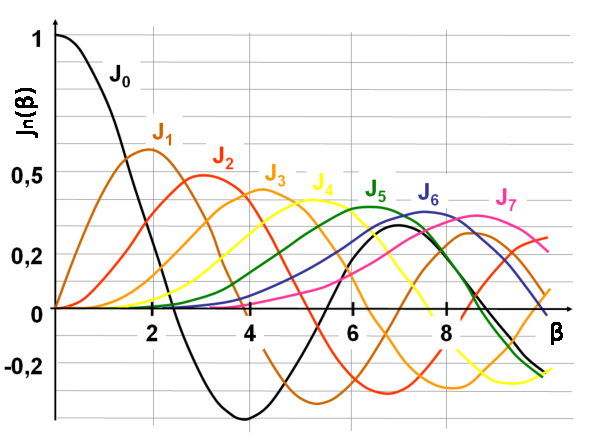
\includegraphics{chapters/06_amplitudenmodulation/figures/besselfunktionen.pdf}
\end{minipage}
\begin{minipage}{.3\linewidth}
	\textbf{Eigenschaften:}\\

	\efbox[linecolor=red]{$J_{-n}(\beta) = (-1)^n\cdot J_n(\beta)$} \\

	\efbox[linecolor=red]{$J_{n-1}(\beta) + J_{n+1}(\beta) = \frac{2n}{\beta} \cdot J_n(\beta)$} \\

	\efbox[linecolor=red]{$ \sum_{n=-\infty}^{\infty} J^2_n (\beta) = 1$} \\

	\efbox[linecolor=red]{$ \beta_n = \Delta T \cdot 2\pi \cdot n \cdot f_c $} \\

	$\Delta T$: Zeitverzögerung bezogen auf Grundschwingung ($f_c$) \\
	$n$: n-te Harmonische \\

	Tabelle Skript S. 74 bzw. 274 ff.
\end{minipage}

\subsubsection{Bandbreite Einton-Winkelmodulation S. 75}
Theoretisch unendliche Bandbreite \\
Praktisch approximation nach Carson: \efbox[linecolor=red]{$B_{ST} = 2 \cdot (\Delta f+f_m) = 2 \cdot (\beta + 1) \cdot \frac{\omega_m}{2\pi}$} (min. \qty{98}{\%} der Signalleistung)\\
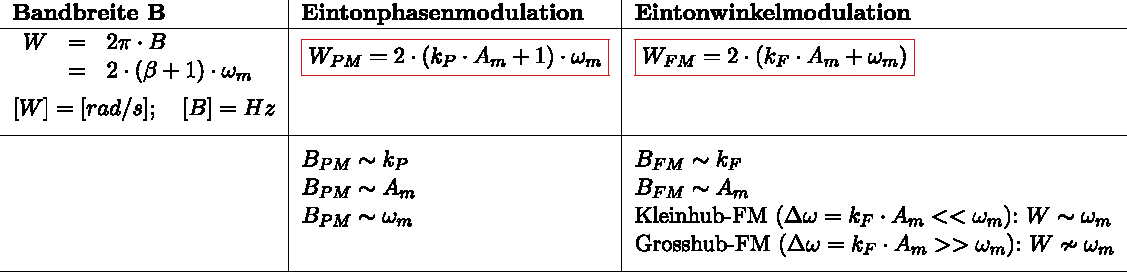
\includegraphics{chapters/06_amplitudenmodulation/figures/Bandbreite.pdf}

\subsubsection[Bandbreite für beliebige m(t)]{Bandbreite für beliebige $m(t)$ S. 75}
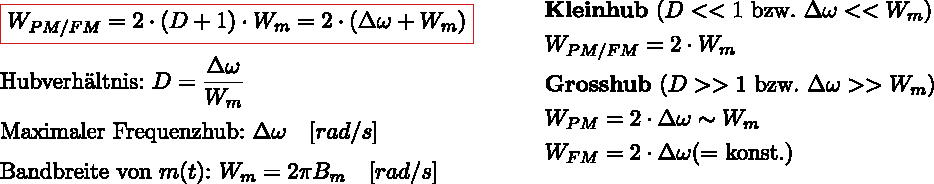
\includegraphics{chapters/06_amplitudenmodulation/figures/bandbreiteBeliebigem.pdf}

\subsubsection{Realisierung}
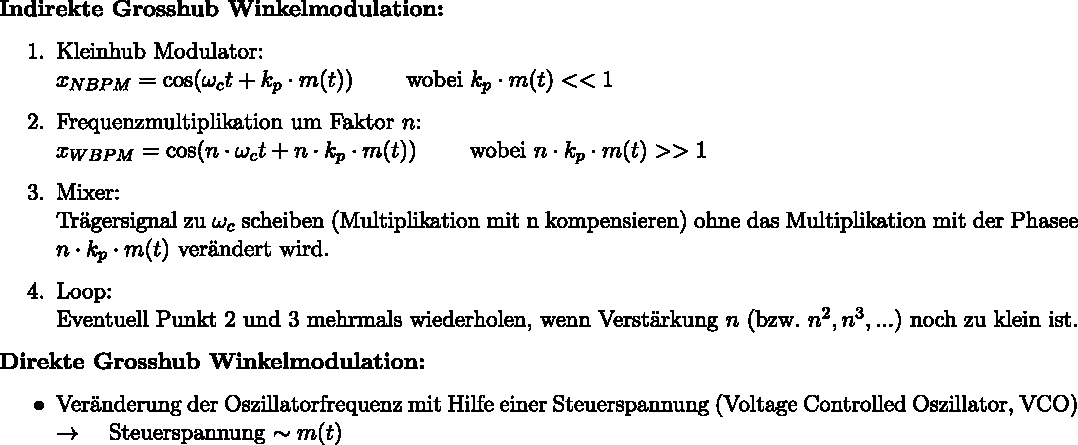
\includegraphics{chapters/06_amplitudenmodulation/figures/realisierungGrosshubWinkelmod.pdf}

\subsubsection{Demodulation}
\paragraph{Phase Locked Loop (PLL)}
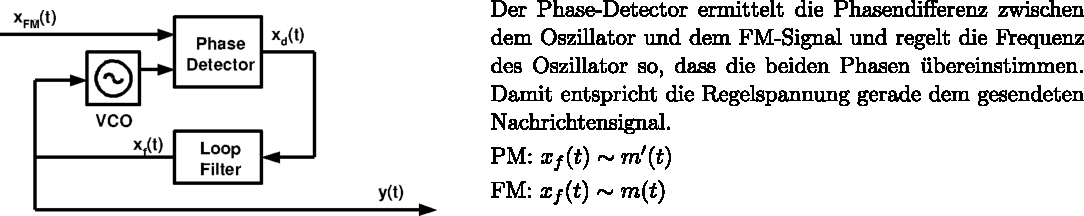
\includegraphics{chapters/06_amplitudenmodulation/figures/PLLdemod.pdf}

\paragraph{Frequenz-Diskriminator}
Die Amplitude des Ausgangssignals eines Frequenz-Diskriminators ist proportional zur Momentanfrequenz des Eingangssignals. $\rightarrow y_d(t) = k_d \cdot \varphi'(t)$ \\
\textbf{PM:} $y_d(t)=k_d\cdot k_P \cdot m'(t)$ \\
\textbf{FM:} $y_d(t) = k_d \cdot k_F \cdot m(t)$

\subsubsection{FM Empfänger S. 77}
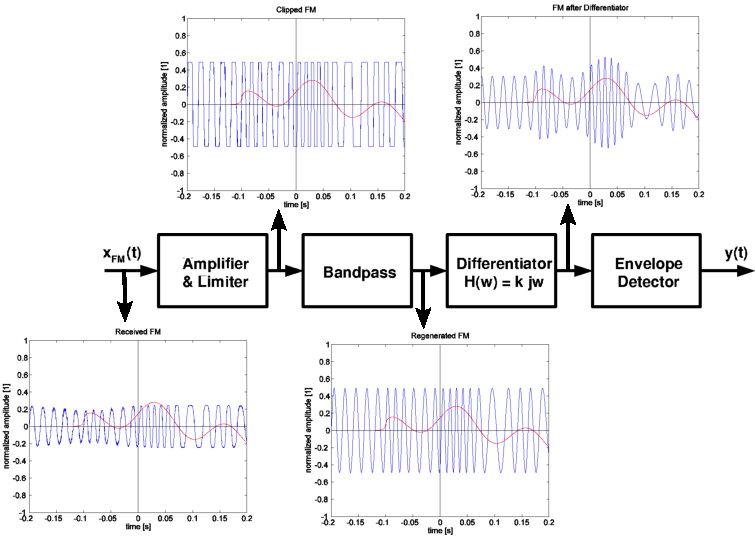
\includegraphics{chapters/06_amplitudenmodulation/figures/FMreceiver.pdf}
